\documentclass[11pt,a4paper]{article}
% ---------------------------------------------------------------------------
%  Stellar Mass Loss Sweeps the Evection Resonance Through Satellite Systems
%  Compile with:  pdflatex evection_sweep && pdflatex evection_sweep
%  (figures are read from ../figures/)
% ---------------------------------------------------------------------------
\usepackage[margin=2.3cm]{geometry}
\usepackage{amsmath,amssymb,bm}
\usepackage{graphicx}
\usepackage{booktabs}
\usepackage[numbers,sort&compress]{natbib}
\usepackage[colorlinks=true,linkcolor=blue!50!black,citecolor=blue!50!black,urlcolor=blue!50!black]{hyperref}
\usepackage{xcolor}
\graphicspath{{../figures/}}

\newcommand{\estar}{e_\star}
\newcommand{\wdot}{\dot\varpi}
\newcommand{\msun}{M_\odot}
\newcommand{\eps}{\varepsilon}
\newcommand{\fJ}{f_{J_2}}
\newcommand{\foct}{f_{\rm oct}}
\newcommand{\dd}{\mathrm{d}}

\title{\textbf{Stellar Mass Loss Sweeps the Evection Resonance Through Satellite Systems:\\ A Universal Eccentricity Imprint and the Fate of Rhea}}
\author{[Author Name]\\[2pt]
{\small [Affiliation]}\\
{\small \texttt{[email]}}}
\date{}

\begin{document}
\maketitle

\begin{abstract}
\noindent
A Sun-like star loses roughly half of its mass on the red-giant and asymptotic giant branches. Every surviving planet then expands its orbit adiabatically and its mean motion falls as $n_p\propto M_\ast^{2}$. We built a dedicated simulator, the \emph{Evection Sweep Lab}, to follow satellites through this phase. It couples an orbit-averaged secular model to direct three-body integrations with stellar mass loss, a semi-analytic solar mass-loss history and Laplace--Lagrange theory for real satellite systems. Our experiments show that stellar mass loss drives the evection resonance $\dot\varpi=n_p$ outward through every satellite system, by a factor $(M_{\ast,i}/M_{\ast,f})^{4/7}$ in semi-major axis. In contrast with inward planetary migration, where moons are captured and destroyed, the sweep runs in the direction in which capture is forbidden. A Hamiltonian normal form explains all regimes we observe. Fast crossings amplify eccentricity as in a Landau--Zener transition, $\langle e_f^2\rangle/e_0^2=2e^{2\Lambda}-1$. Slow crossings obey an exact separatrix-crossing map whose $e_0\to0$ limit is a universal imprint, $\estar=\big[\tfrac{15}{4}(n_p/n_m)\cos^4(\theta/2)/\fJ\big]^{1/2}$, independent of the mass-loss rate. Direct $N$-body integrations revealed a term the quadrupole theory misses. The octupole (parallactic) tide seeds eccentricity even in perfectly circular moons, and with it included the secular model reproduces the $N$-body to $\lesssim2\%$, with errors decreasing as $n_p/n_m\to0$. Applied to the Solar System, Rhea is the only regular moon that is cleanly swept. If its orbit expands by less than $\simeq4\%$ before the Sun dies, Rhea crosses the resonance when the Sun has $0.907\,\msun$ on the upper red-giant branch ($\Lambda\simeq9$--$19$), and its eccentricity rises from $0.001$ to $0.026$--$0.031$, renewing tidal heating by a factor $\sim500$. If Saturn's tidal dissipation is as strong as recent astrometry suggests, the crossing instead falls in the fast AGB superwind and the kick is weak. Rhea's fate is therefore a race between Saturn's tides and the Sun's wind. For exomoons of giant planets around white dwarfs we predict fossil eccentricities of $0.02$--$0.05$ in a well-defined band of orbits.
\end{abstract}

\section{Introduction}

Most planetary systems end around white dwarfs. Before that, their host stars ascend the red-giant branch (RGB) and the asymptotic giant branch (AGB) and shed between a third and four-fifths of their mass in winds \citep{Reimers1975,Bloecker1995,McDonald2015}. The consequences for planets have been studied in depth: orbital expansion \citep{Hadjidemetriou1963,Veras2011}, engulfment and tidal capture \citep{Mustill2012,Schroder2008}, destabilization of multi-planet systems and the delivery of rocky debris that pollutes white-dwarf atmospheres \citep{Zuckerman2003,Veras2016}. A giant planet now transits a white dwarf \citep{Vanderburg2020}, and candidate exomoons are being sought around main-sequence stars \citep{Teachey2018}. The fate of \emph{satellites} through stellar death has received far less attention. The existing studies focus on their liberation by planet--planet scattering after the white dwarf forms \citep{Payne2016}.

The evection resonance occurs when a satellite's apsidal precession rate equals its planet's heliocentric mean motion. It is one of the most consequential resonances in satellite dynamics. It may have shaped the early Earth--Moon system \citep{Touma1998,Cuk2012}, it has been invoked for the inner Saturnian moons \citep{Cuk2016} and Phobos \citep{Vaillant2022}, and it can strip moons from giant planets that migrate inward through their protoplanetary disks \citep{Spalding2016}. Analogues drive eccentric mergers of compact binaries orbiting supermassive black holes \citep{Munoz2022,Bhaskar2022,LiuLai2020}. In every one of these settings the resonance is crossed because the satellite migrates by tides, the inner binary decays by gravitational radiation, or the planet migrates in a disk. We are not aware of any study of the one driver that acts on \emph{every} planetary system that survives its host star: the decline of the planet's mean motion caused by stellar mass loss.

We developed the \emph{Evection Sweep Lab} to follow satellites through post-main-sequence evolution. It is an open simulator that integrates the orbit-averaged dynamics and the full three-body problem side by side and ships with a verification suite (Section~\ref{sec:methods}). Running it, we found four results that we explain and quantify in this paper:
\begin{enumerate}
\item Stellar mass loss sweeps the evection resonance outward through satellite systems in the direction opposite to all previously studied cases, where capture is dynamically forbidden. Instead of destroying moons, the crossing leaves a \emph{universal} eccentricity $\estar$ that depends only on the ratio $n_p/n_m$, the planet's obliquity and the oblateness share of the precession (Sections~\ref{sec:setup}--\ref{sec:results}).
\item When the quadrupole secular theory and the direct $N$-body integrations disagreed by $\sim10\%$, we traced the difference to the octupole term of the stellar tide. This first-order (parallactic) forcing seeds the instability, so even an exactly circular moon acquires an eccentricity of order $\estar$ (Section~\ref{sec:octupole}).
\item A finite integration window biases the linear-regime amplification by $\mathcal O(c/2|\delta_0|)$ unless moons start on the invariant ellipse of the frozen problem. We derive the correct ``proper'' initial conditions (Section~\ref{sec:proper}).
\item In the Solar System the outcome for Saturn's moon Rhea is set by a race between Saturn's tidal dissipation and the Sun's wind (Section~\ref{sec:solar}).
\end{enumerate}

\section{Physical setup and scalings}\label{sec:setup}

\subsection{Adiabatic stellar mass loss}

When the mass-loss timescale $t_M\equiv M_\ast/|\dot M_\ast|$ greatly exceeds the planet's orbital period, a planet on a near-circular orbit conserves its specific angular momentum $\sqrt{GM_\ast a_p}$ and its eccentricity \citep{Hadjidemetriou1963,Veras2011}. Hence
\begin{equation}
a_p M_\ast=\text{const},\qquad n_p=\Big(\frac{GM_\ast}{a_p^3}\Big)^{1/2}\propto M_\ast^{2},\qquad \frac{\dot n_p}{n_p}=-\frac{2}{t_M}.
\label{eq:adiabatic}
\end{equation}
A Sun-like star that ends as a $0.54$--$0.57\,\msun$ white dwarf therefore lengthens the years of its planets by a factor $(M_{\ast,i}/M_{\ast,f})^{2}\simeq3.1$--$3.4$. Saturn's year grows from $29.5$ to about $94$\,yr.

\subsection{Satellite precession and the evection condition}

For a regular satellite of semi-major axis $a_m$, mean motion $n_m$ and eccentricity $e$ orbiting in the equatorial plane of a planet of radius $R_p$ and oblateness $J_2$, the apsidal precession is
\begin{equation}
\dot\varpi=\frac{3}{2}\,n_m J_2\Big(\frac{R_p}{a_m}\Big)^{2}(1-e^2)^{-2}+g_{\rm ext}+\frac{3}{4}\frac{n_p^2}{n_m}\sqrt{1-e^2}\,f_\theta,
\qquad f_\theta=\frac{3\cos^2\theta-1}{2},
\label{eq:precession}
\end{equation}
where $g_{\rm ext}$ collects the contributions of other satellites and of $J_4$, and the last term is the secular precession due to the star. Here $\theta$ is the planet's obliquity. We write $\fJ$ for the fraction of the total precession contributed by $J_2$. The evection resonance is the commensurability
\begin{equation}
\dot\varpi=n_p ,
\label{eq:evection}
\end{equation}
under which the resonant angle $\phi\equiv\varpi-\lambda_p$ is stationary ($\lambda_p$ is the planet's mean longitude).

\subsection{Location and direction of the sweep}

When $J_2$ dominates, Eq.~\eqref{eq:evection} with $e\to0$ defines an evection radius $a_{\rm ev}$ with $a_{\rm ev}^{7/2}\propto n_p^{-1}$. Combining with Eq.~\eqref{eq:adiabatic},
\begin{equation}
a_{\rm ev}\propto n_p^{-2/7}\propto M_\ast^{-4/7},\qquad \frac{a_{\rm ev,f}}{a_{\rm ev,i}}=\Big(\frac{M_{\ast,i}}{M_{\ast,f}}\Big)^{4/7}\simeq1.42\ (1\,\msun\to0.54\,\msun),\quad 2.3\ (3\,\msun\to0.7\,\msun).
\label{eq:sweep}
\end{equation}
Every moon with $a_{\rm ev,i}<a_m<a_{\rm ev,f}$ is crossed. At resonance the tidal small parameter is
\begin{equation}
\eps\equiv\frac{n_p}{n_m}\bigg|_{\rm res}=\frac{3}{2\fJ}\,J_2\Big(\frac{R_p}{a_m}\Big)^{2},
\label{eq:epsres}
\end{equation}
typically $10^{-4}$--$10^{-3}$. The direction of the sweep is the crux of this paper. The ratio $\dot\varpi/n_p$ evolves as
\begin{equation}
\frac{\dd}{\dd t}\ln\frac{\dot\varpi}{n_p}=\frac{2}{t_M}-\frac{7}{2}\frac{\dot a_m}{a_m}.
\label{eq:direction}
\end{equation}
Tidal recession ($\dot a_m>0$), as for the early Moon, decreases $\dot\varpi/n_p$ through unity. So does inward planetary migration, which raises $n_p$. That is the direction in which moons are captured and pumped \citep{Touma1998,Spalding2016}. Stellar mass loss \emph{increases} it. On the upper RGB, $2/t_M\sim3\times10^{-8}$\,yr$^{-1}$ exceeds the tidal term by one to three orders of magnitude for Saturn's moons, depending on Saturn's tidal $Q$. The sweep is therefore driven by the star, and it runs the other way.

\section{Secular theory}\label{sec:theory}

\subsection{Orbit-averaged Hamiltonian}

We use Delaunay variables $(l,L)$, $(g,G)$ for the satellite about the planet, with $L=\sqrt{\mu a_m}$, $G=L\sqrt{1-e^2}$, $\mu=Gm_p$ and $\varpi=g$ in the planar problem. The oblateness term averaged over the satellite's orbit is
\begin{equation}
\langle\mathcal H_{J_2}\rangle=-\frac{\mu J_2R_p^2}{2a_m^3(1-e^2)^{3/2}}.
\end{equation}
The stellar tide in the planet's frame is the expansion $\Phi=-GM_\ast\sum_{\ell\ge2}r^{\ell}P_\ell(\cos\psi)/a_p^{\ell+1}$, where $\psi$ is the angle between the satellite and the star. Averaging over the satellite's mean anomaly with $\langle(r/a)^2\cos2f\rangle=\tfrac52e^2$ and $\langle(r/a)^3\cos f\rangle=-\tfrac52e$, but not over the planet's orbit, gives the quadrupole and octupole terms
\begin{align}
\langle\mathcal H_2\rangle&=-\frac{n_p^2a_m^2}{4}\Big[f_\theta\Big(1+\frac{3}{2}e^2\Big)+\frac{15}{2}\cos^4\!\frac{\theta}{2}\;e^2\cos2\phi\Big],\label{eq:H2}\\
\langle\mathcal H_3\rangle&=-\frac{15}{16}\,n_p^2\,\frac{a_m^3}{a_p}\,\foct(\theta)\;e\cos\phi,\label{eq:H3}
\end{align}
with the obliquity factors derived in Appendix~\ref{app:obliquity},
\begin{equation}
\foct(\theta)=5\big(C_+^3+2C_+C_-^2\big)-4C_+,\qquad C_\pm=\frac{1\pm\cos\theta}{2},
\label{eq:foct}
\end{equation}
normalized so that $\foct(0)=1$. For Saturn ($\theta=26.7^\circ$), $\cos^4(\theta/2)=0.896$ and $\foct=0.48$. Non-resonant harmonics with arguments $2\varpi$ and $2(\varpi+\lambda_p)$ average out near the resonance and are omitted. In the frame rotating with the planet, $\mathcal K=\mathcal H-n_pG$ depends on $\varpi$ only through $\phi$.

\subsection{Equations of motion}

In the non-singular variables $(h,k)=e(\cos\phi,\sin\phi)$, Hamilton's equations become
\begin{equation}
\dot h=-k\,(W-C),\qquad \dot k=h\,(W+C)+F,
\label{eq:hk}
\end{equation}
\begin{equation}
W=\dot\varpi(e)-n_p,\qquad C=\frac{15}{4}\frac{n_p^2}{n_m}\sqrt{1-e^2}\cos^4\!\frac{\theta}{2},\qquad F=\frac{15}{16}\frac{n_p^2}{n_m}\frac{a_m}{a_p}\foct(\theta)\sqrt{1-e^2}.
\label{eq:WCF}
\end{equation}
The quadrupole couples $h$ and $k$ parametrically. The octupole enters as a constant forcing of $k$. These are the equations integrated by the secular module of the simulator, with $n_p(t)$, $a_p(t)$ and optional tidal damping ($\dot h\to\dot h-h/\tau_e$, $\dot k\to\dot k-k/\tau_e$).

\subsection{Normal form and the absence of capture}

Close to resonance we measure time in units of $1/n_p$ and define the detuning $\delta\equiv\dot\varpi_0/n_p-1+\tfrac34\eps f_\theta$, where $\dot\varpi_0$ is the precession at $e=0$. With $x=1-\sqrt{1-e^2}\simeq e^2/2$, the quadrupole problem reduces to the second fundamental model of resonance \citep{Henrard1982},
\begin{equation}
K(x,\phi)=\delta\,x+\beta x^2+c\,x\cos2\phi,\qquad c=\frac{15}{4}\eps\cos^4\!\frac{\theta}{2},\qquad \beta=2\fJ .
\label{eq:normal}
\end{equation}
Its fixed points lie at $\phi=0,\pi$, $x_1=-(\delta+c)/2\beta$ (hyperbolic) and at $\phi=\pm\pi/2$, $x_2=(c-\delta)/2\beta$ (elliptic). The origin is unstable inside the \emph{parametric band}
\begin{equation}
|\delta|<c,\qquad \sigma=\sqrt{c^2-\delta^2},
\label{eq:band}
\end{equation}
where $\sigma$ is the growth rate of $e$. Under mass loss, Eq.~\eqref{eq:adiabatic} gives
\begin{equation}
\frac{\dd\delta}{\dd\tau}=\frac{2}{n_pt_M}>0 .
\label{eq:deltadot}
\end{equation}
Figure~\ref{fig:portraits} shows the phase portraits during such a sweep. For $\delta<-c$ the moon sits in an inner circulation region bounded by a separatrix that also encloses two resonant lobes. As $\delta$ increases, the inner region, the resonant lobes and the islands at $x_2$ \emph{all shrink}. By Henrard's criterion \citep{Henrard1982,Neishtadt1975}, the probability of capture into a region whose area decreases is zero. The moon is expelled into the outer circulation region and carries away the area enclosed by the separatrix at that moment. In the opposite direction, which is the classical case, the islands grow and capture is certain for small $e_0$. Our simulations confirm both behaviours (Section~\ref{sec:results}, Fig.~\ref{fig:timeseries}d).

\subsection{Fast crossings: Landau--Zener amplification}\label{sec:LZ}

For $e\ll\estar$ the problem is linear. With $\zeta=h+ik$ and $F=0$, Eq.~\eqref{eq:hk} becomes $\dot\zeta=i\delta\zeta+ic\zeta^*$. Setting $\zeta=w\exp(i\!\int\!\delta\,\dd t)$ gives $\dot w=ic\,w^*e^{-2i\int\delta\,\dd t}$. This is the Landau--Zener problem \citep{Landau1932,Zener1932} with the product of the couplings reversed in sign. The final state is a Bogoliubov transformation $w_f=\alpha w_0+\beta' w_0^*$ with $|\alpha|^2-|\beta'|^2=1$ and $|\alpha|^2=e^{2\Lambda}$. Averaging over the initial phase,
\begin{equation}
\frac{\langle e_f^2\rangle_{\phi_0}}{e_0^2}=2e^{2\Lambda}-1,\qquad e^{\Lambda}-\sqrt{e^{2\Lambda}-1}\le\frac{e_f}{e_0}\le e^{\Lambda}+\sqrt{e^{2\Lambda}-1},
\label{eq:LZ}
\end{equation}
where the adiabaticity parameter is the integrated growth $\int\sigma\,\dd\tau=\pi c^2/(2\dot\delta)$:
\begin{equation}
\Lambda=\frac{\pi c^2}{2\,\dd\delta/\dd\tau}=\frac{225\pi}{64}\Big(\frac{n_p}{n_m}\Big)^{2}\cos^8\!\frac{\theta}{2}\;n_pt_M .
\label{eq:Lambda}
\end{equation}
Equation~\eqref{eq:Lambda} is the single number that decides how violent a crossing is. For Rhea on the upper RGB, $\Lambda\simeq9$--$19$.

\subsection{Slow crossings: the adiabatic jump map and the universal imprint}\label{sec:adiabatic}

For $\Lambda\gg\ln(\estar/e_0)$ the action $J=\oint x\,\dd\phi$ is conserved except at the separatrix crossing. Writing $\delta=-qc$ ($q\ge1$), the areas of the inner region and of the region enclosed by the outer separatrix follow from Eq.~\eqref{eq:normal} in closed form (Appendix~\ref{app:areas}):
\begin{equation}
A_{\rm in,out}(q)=\frac{c}{\beta}\Big[\pi q\mp2\sqrt{q-1}\mp2q\arcsin q^{-1/2}\Big].
\label{eq:areas}
\end{equation}
The moon leaves the inner region when $A_{\rm in}(q)=\pi e_0^2$ and lands on the outer region with $J=A_{\rm out}(q)$, so that
\begin{equation}
e_0^2=\frac{\estar^2}{2\pi}\Big[\pi q-2\sqrt{q-1}-2q\arcsin q^{-1/2}\Big],\qquad
e_f^2=\frac{\estar^2}{2\pi}\Big[\pi q+2\sqrt{q-1}+2q\arcsin q^{-1/2}\Big],
\label{eq:jumpmap}
\end{equation}
with
\begin{equation}
\estar^2=\frac{2c}{\beta}=\frac{15}{4}\,\frac{n_p}{n_m}\,\frac{\cos^4(\theta/2)}{\fJ}.
\label{eq:estar}
\end{equation}
Equation~\eqref{eq:jumpmap} has two limits:
\begin{equation}
e_f\xrightarrow{\;e_0\to0\;}\estar,\qquad e_f\simeq e_0+\frac{2\sqrt2}{\pi}\,\estar\quad(e_0\gg\estar).
\label{eq:limits}
\end{equation}
Every adiabatically swept moon is left with an eccentricity of order $\estar$, independent of how fast or how slowly the star lost its mass. Using Eq.~\eqref{eq:epsres}, the imprint can be written in terms of planetary properties alone:
\begin{equation}
\estar=\Big(\frac{45J_2}{8}\Big)^{1/2}\frac{R_p}{a_m}\,\frac{\cos^2(\theta/2)}{\fJ}.
\label{eq:estarJ2}
\end{equation}
For Rhea, $\estar=0.0354$. For a Jupiter analogue at 5.2\,AU, $\estar$ falls from $0.043$ to $0.031$ across the swept band.

\subsection{Octupole seeding of circular moons}\label{sec:octupole}

In the quadrupole problem a perfectly circular orbit stays circular forever, because the origin is a fixed point. The octupole forcing $F$ of Eq.~\eqref{eq:WCF} removes this degeneracy. Far from resonance it maintains a forced eccentricity $h_f=-F/(W+C)$, and its passage through the band delivers a stationary-phase kick of size $F\sqrt{2\pi/\dot\delta}$. In units of $\estar$ this is
\begin{equation}
\frac{e_{\rm seed}}{\estar}\simeq2\xi\sqrt{\Lambda},\qquad \xi\equiv\frac{a_m}{a_p}\,\frac{\foct(\theta)}{4\cos^4(\theta/2)\,\estar},
\label{eq:seed}
\end{equation}
which is subsequently amplified by a factor between the rms and the maximum gains of Eq.~\eqref{eq:LZ}. For Rhea, $a_m/a_p=3.3\times10^{-4}$ at the crossing and $\xi\simeq1.3\times10^{-3}$. This is small but sufficient. Section~\ref{sec:solar} shows that a circular Rhea still ends at $e\simeq0.024$--$0.029$.

\section{Methods: the Evection Sweep Lab}\label{sec:methods}

The simulator is an open-source Python package (\texttt{evection\_lab}; NumPy, SciPy and Matplotlib, with optional Numba compilation of the $N$-body kernel) that provides the analytic theory, the secular and direct integrators, the stellar and satellite models, an interactive laboratory and the verification suite. An equivalent JavaScript engine powers a browser version. The two implementations agree to the precision of their integrators: the $J_2$ precession test agrees to twelve significant figures, and every entry of the verification suite agrees to four or more.

\subsection{Secular integrator}

Equations~\eqref{eq:hk}--\eqref{eq:WCF} are integrated for ensembles of initial phases with an adaptive Dormand--Prince 5(4) scheme \citep{Dormand1980} at relative tolerance $10^{-10}$ (JavaScript), and with an 8th-order Dormand--Prince scheme in SciPy (Python). In generic runs, time is measured in units of $1/n_{p,\rm res}$ and $n_p=\exp(-t/\tau_n)$ with $\tau_n=2\Lambda/(\pi c^2)$, so that Eq.~\eqref{eq:Lambda} holds exactly. The window runs from $\delta=-K_0c$ to $\delta=+K_1c$ with $K_1=12$. The final eccentricity is the rms over the last 15\% of the run, which removes the residual $\mathcal O(c/\delta)$ modulation. For eccentric moons the window must open inside the inner separatrix, which requires $K_0>(1+\sqrt2\,e_0/\estar)^2$; we use $K_0=\max[7,(1+1.5e_0/\estar)^2+5]$.

\subsection{Proper initial conditions}\label{sec:proper}

Our first linear-regime experiments returned gains that fluctuated by $\pm7\%$ as $K_0$ was changed ($3.48$, $4.01$ and $3.74$ for $K_0=7$, $8$, $15$ at $\Lambda=1$, against $3.71$ from Eq.~\eqref{eq:LZ}). The cause is that a circle $|\zeta|=e_0$ is not an invariant curve of the frozen linear problem at finite detuning. The invariant curves are the ellipses
\begin{equation}
(W+C)h^2+(W-C)k^2=\text{const},\qquad \frac{\text{semi-axis}_h}{\text{semi-axis}_k}=A^2,\quad A=\Big|\frac{W-C}{W+C}\Big|^{1/4},
\label{eq:proper}
\end{equation}
and their mismatch with the circle mixes the Bogoliubov modes with weight $\simeq c/2|\delta_0|$. We therefore start moons on the invariant ellipse of area $\pi e_0^2$, offset by the octupole-forced eccentricity $h_f$. With these proper initial conditions the gain becomes independent of the window ($3.746$, $3.733$, $3.745$, $3.733$ for four windows), and the residual $0.6$--$0.9\%$ excess over Eq.~\eqref{eq:LZ} vanishes as $\eps\to0$. The $N$-body comparisons use osculating initial conditions in both codes, because that is what a direct integration starts from.

\subsection{Direct three-body integrations with mass loss}

The direct module integrates the restricted planar three-body problem in the planet-centred frame:
\begin{equation}
\ddot{\bm r}=-\frac{Gm_p}{r^3}\bm r-\frac{3}{2}\frac{Gm_pJ_2R_p^2}{r^5}\bm r+GM_\ast(t)\Big[\frac{\bm X}{X^3}-\frac{\bm X+\bm r}{|\bm X+\bm r|^3}\Big],\qquad
\ddot{\bm X}=-\frac{G(M_\ast+m_p)}{X^3}\bm X,
\label{eq:nbody}
\end{equation}
where $\bm X$ is the planet's heliocentric position. The tide is the full, unexpanded expression; a switch replaces it by its quadrupole part $GM_\ast X^{-3}[3(\bm r\cdot\hat{\bm X})\hat{\bm X}-\bm r]$. Mass is lost isotropically as $M_\ast+m_p=(M_{\ast,0}+m_p)\,e^{-t/2\tau}$, which gives $n_p\propto e^{-t/\tau}$ through Eq.~\eqref{eq:adiabatic}. The planet's orbit is integrated self-consistently, not prescribed. We use units $G=M_{\ast,0}=a_{p,0}=1$ and $m_p=10^{-3}$, set $R_p=a_m/3$, and choose $J_2$ so that Eq.~\eqref{eq:evection} is met at $\delta=0$. We use a fourth-order symplectic composition of drift--kick--drift leapfrogs \citep{Yoshida1990} in extended phase space, so the explicit time dependence of $M_\ast$ is handled exactly, with 200 steps per satellite orbit. The eccentricity is the osculating Keplerian eccentricity vector averaged over each satellite orbit, which removes the $J_2$-induced short-period offset. Two built-in tests pass: the measured $J_2$ precession agrees with Eq.~\eqref{eq:precession} to $2\times10^{-4}$, and the adiabatic invariant $a_p(M_\ast+m_p)$ is conserved to $<10^{-5}$.

\subsection{Solar mass-loss history}

We follow the Sun from the base of the RGB with a semi-analytic model. On the RGB we use the degenerate-core relations of \citet{Rappaport1995},
\begin{equation}
\frac{L}{L_\odot}=\frac{10^{5.3}\mu_c^{6}}{1+10^{0.4}\mu_c^{4}+10^{0.5}\mu_c^{5}},\qquad \frac{R}{R_\odot}=\frac{3.7\times10^{3}\mu_c^{4}}{1+\mu_c^{3}+1.75\mu_c^{4}},\qquad \mu_c=\frac{M_c}{\msun},
\end{equation}
with core growth $\dot M_c=L/(XQ_H)$ ($X=0.70$, $Q_H=6.0\times10^{18}$\,erg\,g$^{-1}$) up to the helium flash at $M_c=0.47\,\msun$. Mass is lost in a Reimers wind,
\begin{equation}
\dot M_\ast=-4\times10^{-13}\,\eta\,\frac{(L/L_\odot)(R/R_\odot)}{M_\ast/\msun}\ \msun\,{\rm yr^{-1}},
\end{equation}
with $\eta=0.477$ as calibrated on globular clusters \citep{McDonald2015}; we also test $\eta=0.3$ and $0.7$. A red-clump phase of $1.1\times10^8$\,yr follows ($L=45L_\odot$, $R=10R_\odot$). On the AGB we use $L=59250(M_c/\msun-0.495)L_\odot$ \citep{Wood1981} and $T_{\rm eff}=3300$\,K, and take the larger of the Reimers wind and the superwind of \citet{Bloecker1995} with $\eta_B=0.05$. The model ends with a $0.561\,\msun$ white dwarf for $\eta=0.477$ ($0.572$ and $0.529$ for $\eta=0.3$, $0.7$), with $0.777\,\msun$ at the RGB tip. Both values are consistent with detailed solar models \citep{Schroder2008}. Only the local value of $t_M$ at the crossing enters Eq.~\eqref{eq:Lambda}.

\subsection{Real satellite systems}

For the regular moons of Mars, Jupiter, Saturn, Uranus and Neptune we compute the free apsidal eigenfrequencies from classical Laplace--Lagrange theory with $J_2$, $J_4$, the $J_2^2$ correction, the mutual secular coupling and the solar quadrupole \citep{MurrayDermott1999},
\begin{equation}
A_{jj}=n_j\Big[\tfrac32J_2\big(\tfrac{R_p}{a_j}\big)^2-\tfrac98J_2^2\big(\tfrac{R_p}{a_j}\big)^4-\tfrac{15}{4}J_4\big(\tfrac{R_p}{a_j}\big)^4+\tfrac14\sum_{k\ne j}\tfrac{m_k}{m_p}\alpha_{jk}\bar\alpha_{jk}b^{(1)}_{3/2}(\alpha_{jk})\Big]+\tfrac34\tfrac{n_p^2}{n_j}f_\theta,
\end{equation}
with $A_{jk}=-\tfrac14n_j(m_k/m_p)\alpha_{jk}\bar\alpha_{jk}b^{(2)}_{3/2}(\alpha_{jk})$. We use the gravity fields of \citet{Jacobson2006} and \citet{Iess2018}. As a check, the code returns a free apsidal period of $705$\,yr for Titan, consistent with the observed value of $\simeq703$\,yr. For each mode we solve $g_j(M_\ast)=n_{p,0}(M_\ast/\msun)^2$ for the crossing mass.

\section{Results}\label{sec:results}

\subsection{Through the crossing}

Figure~\ref{fig:timeseries} shows ensembles of 24 initial phases at $\eps=3\times10^{-3}$ and $e_0=0.01\estar$. For $\Lambda=1$ (panel a) the eccentricity grows only inside the band and the final values follow the Landau--Zener spread. For $\Lambda=8$ most members reach the separatrix and leave with $e_f\simeq0.6$--$0.7\estar$. For $\Lambda=128$ all members converge on $e_f=0.957\estar$, the universal imprint. Panel (d) reverses the sweep. Every member is captured and pumped along the island to $2.37\estar$, which matches the rms of the exact island centre over the averaging window (2.374) to 0.02\%. The asymmetry between panels (c) and (d) is the central result of this paper: stellar mass loss marks satellites but cannot capture them.

\subsection{The universal transfer function}

We mapped the mean final eccentricity over a grid of 18 values of $\Lambda$ ($0.125$--$256$) and 16 values of $e_0/\estar$ ($10^{-5}$--$3$), with 32 phases each (Fig.~\ref{fig:transfer}). Because $\estar$ and $\Lambda$ absorb all physical parameters, this one map applies to any moon, planet and star in the quadrupole limit. The linear prediction Eq.~\eqref{eq:LZ} holds until $e_f$ approaches $\sim0.3\estar$. At $\Lambda=256$ the simulated means agree with the jump map Eq.~\eqref{eq:jumpmap} to $0.1$--$1.1\%$ for all $0.1\le e_0/\estar\le3$ (Fig.~\ref{fig:transfer}b). For $e_0\to0$ the plateau $\estar$ is approached slowly: $e_f/\estar=0.828$, $0.895$, $0.937$ at $\Lambda=64$, $128$, $256$ for $e_0=10^{-5}\estar$. The orbit spends a time $\propto\ln(\estar/e_0)/\sigma$ near the hyperbolic origin, where adiabaticity fails, and so exits the band late, when the separatrix area has already shrunk.

\subsection{Validation against direct integrations}

Figure~\ref{fig:nbody} compares the two codes. A single trajectory (panel a; $\eps=0.005$, $\Lambda=8$) is reproduced in detail, with $e_f/\estar=0.761$ ($N$-body) against $0.794$ (secular). Ensemble means at $\eps=0.005$ agree across the full range of $\Lambda$: $0.090/0.090$, $0.166/0.163$, $0.373/0.374$, $0.640/0.633$, $0.792/0.782$, $0.898/0.895$ and $0.952/0.959$ for $\Lambda=0.5$--$32$. Panel (c) shows that the residual differences in the linear regime decrease from 18\% at $\eps=0.02$ to 5\% at $\eps=0.01$ and to $\lesssim2\%$ for $\eps\le0.005$, both for the full tide against the quadrupole-plus-octupole theory and for the quadrupole tide against the quadrupole theory. These are the higher-order corrections in $\eps$ familiar from lunar theory; between $\eps=0.02$ and $0.01$ they fall roughly as $\eps^2$, and they are negligible for real moons ($\eps\sim10^{-4}$). For eccentric moons at $\Lambda=16$ the codes give $1.384$ and $1.392$ for $e_0=0.5\estar$ (adiabatic map: $1.419$), $1.892$ and $1.908$ for $e_0=\estar$ (adiabatic map: $1.908$), and $2.856$ and $2.942$ for $e_0=2\estar$ (adiabatic map: $2.903$).

The octupole term was discovered through this comparison. With the quadrupole theory alone, the full-tide integrations disagreed phase by phase by up to a factor of two at $\eps=0.01$. They broke the $\phi\to\phi+\pi$ symmetry of Eq.~\eqref{eq:normal}, and they excited exactly circular moons ($e_f=0.047$, i.e.\ $0.24\,\estar$, at $\eps=0.01$ and $\Lambda=2$, where the quadrupole theory predicts zero). Switching the integrator to a quadrupole-only tide restored agreement to $\sim5\%$, which isolated the $\ell=3$ term. Adding Eq.~\eqref{eq:H3} to the secular model reproduced the full-tide results.

\subsection{Circular moons}

Figure~\ref{fig:octupole} shows initially circular moons for octupole strengths $\xi=3\times10^{-4}$--$3\times10^{-2}$. At small $\Lambda$, $e_f$ lies within the band predicted by Eq.~\eqref{eq:seed} times the Landau--Zener gains. At large $\Lambda$ every curve converges on $\estar$, slightly exceeded for large $\xi$ because the forced eccentricity adds to the free one. Direct integrations of circular moons ($\eps=0.005$) agree with the secular model, for example $e_f/\estar=0.014/0.014$ at $\Lambda=0.5$ and $0.041/0.041$ at $\Lambda=1$. Physically, the parallactic term guarantees that no moon escapes the imprint by being tidally circularized beforehand.

\section{Application I: the Solar System as the Sun dies}\label{sec:solar}

\subsection{Which moons are swept}

Figure~\ref{fig:sweep} and Table~\ref{tab:moons} compare each planet's lengthening year with the free apsidal periods of its moons. Five modes are crossed before the Sun becomes a white dwarf. Phobos is irrelevant: it will spiral into Mars within $\sim50$\,Myr. Europa is crossed on the AGB ($M_\ast=0.631\,\msun$), but it is locked in the Laplace resonance and needs a resonant secular theory that we do not attempt. Umbriel and Titania are crossed, but Uranus's $98^\circ$ obliquity suppresses the evection coupling by $\cos^8(\theta/2)\simeq0.03$ and gives $\Lambda<0.01$; their eccentricities change negligibly. Rhea is the one clean case. Its precession is 93\% due to Saturn's $J_2$, it is in no mean-motion resonance, and it is crossed on the slow RGB wind.

\begin{table}[t]
\centering
\caption{Satellites whose free apsidal mode is crossed by the evection resonance before the Sun becomes a white dwarf (Laplace--Lagrange theory, present orbits). $P_\varpi$ is the free apsidal period, $M_x$ the solar mass at the crossing, and $\Lambda$ is given for $\eta=0.3/0.477/0.7$.}
\label{tab:moons}
\small\setlength{\tabcolsep}{4pt}
\begin{tabular}{llrrrrrrrl}
\toprule
Planet & Moon & $a_m/R_p$ & $P_\varpi$ (yr) & $\fJ$ & $M_x/\msun$ & $\eps$ & $\estar$ & $\Lambda$ & Note \\
\midrule
Mars    & Phobos   & 2.76  & 2.26   & 1.00 & 0.913 & $3.9\times10^{-4}$ & 0.036 & 207/315/447 & decays first \\
Jupiter & Europa   & 9.39  & 29.75  & 0.77 & 0.631 & $3.3\times10^{-4}$ & 0.040 & 0.18/0.49/782 & Laplace MMR \\
Saturn  & Rhea     & 8.74  & 35.84  & 0.93 & 0.907 & $3.5\times10^{-4}$ & 0.035 & 8.8/13.3/18.8 & clean case \\
Uranus  & Umbriel  & 10.41 & 129.1  & 0.55 & 0.807 & $8.8\times10^{-5}$ & 0.011 & $<0.01$ & $\theta=98^\circ$ \\
Uranus  & Titania  & 17.07 & 204.7  & 0.16 & 0.641 & $1.2\times10^{-4}$ & 0.023 & $\le0.52$ & $\theta=98^\circ$ \\
\bottomrule
\end{tabular}
\end{table}

\subsection{Rhea's crossing}

Rhea's free mode has a period of $35.84$\,yr today against Saturn's $29.46$\,yr year. The two coincide when $M_\ast=0.9066\,\msun$, about $490$\,Myr after the Sun leaves the base of the RGB, when its luminosity is $460$--$1220\,L_\odot$ depending on $\eta$ ($718\,L_\odot$ for $\eta=0.477$; Fig.~\ref{fig:rhea}a). There $t_M=4.7$, $7.2$ and $10.2\times10^7$\,yr for $\eta=0.3$, $0.477$, $0.7$, giving $\Lambda=8.8$, $13.3$ and $18.8$. Monte Carlo runs over 64 initial phases (Table~\ref{tab:rhea}, Fig.~\ref{fig:rhea}) give a final eccentricity of $0.026$--$0.031$ for a free eccentricity $e_0=10^{-3}$, and $0.024$--$0.029$ even for a circular start. Rhea's observed eccentricity of $0.00126$ is mostly forced by Titan: our secular theory gives a forced component of $9.7\times10^{-4}$, so its free eccentricity lies between about $3\times10^{-4}$ and $2\times10^{-3}$. The outcome hardly depends on this, because the crossing is close to adiabatic.

Saturn's obliquity is not fixed. Titan's migration may drive it to $55$--$65^\circ$ within 5\,Gyr \citep{Saillenfest2021a,Saillenfest2021b}. A larger obliquity weakens the coupling as $\cos^8(\theta/2)$. At $\theta=60^\circ$ we find $\Lambda=3.5$--$7.4$ and $e_f=0.014$--$0.021$ ($e_0=10^{-3}$), still a tenfold increase over today.

\begin{table}[t]
\centering
\caption{Rhea's eccentricity after the crossing (mean and 5--95\% range over 64 initial phases), for its present orbit, octupole included. Upper rows: free $e_0=10^{-3}$; lower rows: initially circular.}
\label{tab:rhea}
\begin{tabular}{lccc}
\toprule
 & $\theta=26.7^\circ$ (today) & $\theta=45^\circ$ & $\theta=60^\circ$ \\
\midrule
$\estar$ & 0.0354 & 0.0319 & 0.0280 \\
$\eta=0.30$  & $0.0264\,[0.021,0.029]$ & $0.0209\,[0.014,0.024]$ & $0.0138\,[0.005,0.018]$ \\
$\eta=0.477$ & $0.0290\,[0.025,0.031]$ & $0.0240\,[0.020,0.026]$ & $0.0179\,[0.012,0.021]$ \\
$\eta=0.70$  & $0.0305\,[0.027,0.032]$ & $0.0260\,[0.023,0.028]$ & $0.0205\,[0.015,0.023]$ \\
\midrule
$\eta=0.30$, $e_0=0$  & 0.0236 & 0.0122 & 0.0079 \\
$\eta=0.477$, $e_0=0$ & 0.0272 & 0.0188 & 0.0147 \\
$\eta=0.70$, $e_0=0$  & 0.0294 & 0.0223 & 0.0185 \\
\bottomrule
\end{tabular}
\end{table}

\subsection{Tides versus wind}

Rhea will migrate outward before the Sun dies. Astrometry suggests that Saturn's dissipation at Rhea's tidal frequency is an order of magnitude stronger than at the inner moons ($Q\sim300$; \citealt{Lainey2017}), in line with resonance locking \citep{Fuller2016,Lainey2020}. We re-solved the Laplace--Lagrange problem for Rhea's orbit expanded by a factor $f$ (Titan held fixed). The crossing survives for any $f\le1.6$, because Titan's growing secular contribution compensates the weaker $J_2$ term. At such expansions Rhea would also meet mean-motion commensurabilities with Titan (3:1 at $f\simeq1.11$, 5:2 at $f\simeq1.26$ if Titan stays put), which we do not model. It does move to lower solar mass, however: $M_x=0.879$, $0.853$, $0.805$, $0.712$ and $0.618\,\msun$ for $f=1.02$, $1.04$, $1.08$, $1.18$ and $1.36$. Figure~\ref{fig:race} shows the consequence. For $f\lesssim1.04$ the crossing occurs on the slow RGB wind and Rhea receives the full imprint. For $f\gtrsim1.1$ it falls on the AGB superwind, where $t_M\sim10^6$\,yr and $\Lambda<1$, and Rhea leaves with $e\simeq0.001$--$0.003$. Narrow windows of full excitation appear where $M_x$ coincides with the red clump, whose weak wind makes the crossing adiabatic again. For constant $Q$, the expansion over the next $7.6$\,Gyr is
\begin{equation}
f^{13/2}=1+\frac{13}{2}\frac{\Delta t}{\tau_0},\qquad \tau_0^{-1}=3\frac{k_2}{Q}\frac{m_m}{M_p}\Big(\frac{R_p}{a_m}\Big)^5n_m,
\label{eq:migration}
\end{equation}
which gives $f=1.36$, $1.18$, $1.08$ and $1.04$ for $Q=300$, $10^3$, $3\times10^3$ and $7\times10^3$ ($k_2=0.39$). Rhea receives the full imprint only if Saturn's effective $Q$ at Rhea's frequency stays above $\sim7\times10^3$ for the next 7.6\,Gyr. If the strong dissipation measured today persists, Rhea crosses during the superwind and is only mildly perturbed. Moons of white-dwarf planets offer a natural test of tidal theory in this sense: the eccentricities they retain record how far they migrated before their star died.

\subsection{Renewed tidal heating}

A Rhea with $e=0.029$ dissipates
\begin{equation}
\dot E=\frac{21}{2}\frac{k_2}{Q}\frac{GM_p^2R_m^5n_me^2}{a_m^6}\simeq3.7\Big(\frac{k_2/Q}{10^{-4}}\Big)\ {\rm GW},
\label{eq:heating}
\end{equation}
about 500 times its present tidal power. The eccentricity damps on
\begin{equation}
\tau_e=\frac{4}{63}\frac{Q}{k_2}\frac{m_m}{M_p}\Big(\frac{a_m}{R_m}\Big)^5\frac{1}{n_m}\simeq0.8\Big(\frac{k_2/Q}{10^{-4}}\Big)^{-1}\ {\rm Gyr},
\label{eq:damping}
\end{equation}
so the heating persists well into the white-dwarf phase. For comparison, the chondritic radiogenic heating of Rhea's rocky component is of order a few GW today and will have decayed severalfold by then.

\section{Application II: exomoons around white dwarfs}\label{sec:exo}

Equation~\eqref{eq:estarJ2} and the transfer function predict the imprint for any satellite system. Figure~\ref{fig:exo} shows moons of a Jupiter analogue ($J_2=0.0147$, $R_p=R_{\rm J}$) around a $1\,\msun$ star ($\eta=0.477$). For main-sequence orbits $a_p=3$, $5.2$, $10$ and $20$\,AU the swept bands are $a_m/R_p=5.3$--$7.3$, $6.7$--$9.3$, $8.9$--$12.3$ and $11.9$--$16.6$, with $\estar=0.054$--$0.017$. In each band the inner part ($a_m/R_p<6.8$, $8.1$, $10.3$ and $13.8$ respectively) is crossed on the RGB with $\Lambda>3$ and retains $e_f\simeq0.4$--$1.0\,\estar$ (for $e_0=10^{-3}$). The outer part is crossed during the superwind and is only weakly perturbed. More massive progenitors sweep wider bands, by a factor up to $2.3$ for $3\,\msun$ (Eq.~\ref{eq:sweep}). Because they lose most of their mass in the superwind, we expect their imprint to be confined to the part of the band crossed on the RGB; quantifying this needs detailed stellar tracks. Three consequences follow:
\begin{itemize}
\item \emph{Fossil eccentricities.} White-dwarf satellite systems should show eccentricities of a few per cent in a band whose inner edge sits at the main-sequence evection radius, a signature that no other post-main-sequence process produces.
\item \emph{Renewed heating.} Icy moons in the band are tidally reheated (Eq.~\ref{eq:heating}) for $\sim0.1$--$1$\,Gyr after the star dies, which bears on the possibility of subsurface oceans around white dwarfs.
\item \emph{Survival.} Unlike inward migration \citep{Spalding2016}, stellar mass loss never destroys a moon through evection, because $e_f\lesssim\estar+e_0\ll1$.
\end{itemize}

\section{Discussion and limitations}

Our models are planar apart from the obliquity factors. They assume a single dominant free mode, a constant planetary $J_2$ and $R_p$, adiabatic and isotropic mass loss, and no planet--planet scattering or stellar tides on the planet. Anisotropic winds and the planet's thermal inflation by the giant star would change $J_2R_p^2$ by a few per cent, shifting the crossing slightly but not the imprint, which depends on $J_2$ only through $\eps$. Satellites in mean-motion resonance (the Galilean moons, Enceladus--Dione) need a resonant secular theory. Inclination analogues (ivection) and the Laplace-surface instability of high-obliquity planets \citep{Tremaine2009} are also swept by mass loss and deserve study. The semi-analytic stellar model is calibrated but simple, and Fig.~\ref{fig:race} shows that the outcome depends sharply on where the crossing falls relative to the RGB tip and the red clump. Detailed stellar evolution tracks would sharpen the Rhea prediction, but not the theory.

\section{Conclusions}

\begin{enumerate}
\item Stellar mass loss sweeps the evection resonance outward through every surviving satellite system, by $(M_{\ast,i}/M_{\ast,f})^{4/7}$ in semi-major axis, in the direction in which capture is forbidden (Eqs.~\ref{eq:sweep}, \ref{eq:direction}).
\item A Hamiltonian normal form gives the full outcome: Landau--Zener amplification for fast crossings (Eq.~\ref{eq:LZ}), an exact jump map for slow ones (Eq.~\ref{eq:jumpmap}), and a universal imprint $\estar$ independent of the mass-loss rate (Eq.~\ref{eq:estar}).
\item Direct integrations exposed octupole (parallactic) seeding, which excites even circular moons, and a start-up bias that we remove with proper initial conditions. With both, the secular model matches the $N$-body to $\lesssim2\%$.
\item Rhea is the Solar System's only clean case. It gains $e\simeq0.03$ on the upper RGB if Saturn's $Q\gtrsim7\times10^3$, and only $e\simeq0.001$--$0.003$ if today's strong dissipation persists.
\item Moons of giant planets around white dwarfs should carry fossil eccentricities of $0.02$--$0.05$ in a predictable band of orbits.
\end{enumerate}

\section*{Code and data availability}
The Evection Sweep Lab is publicly available at \url{https://github.com/Proryon29/evection-lab}. The repository contains the Python package, the campaign and figure scripts, every data file used here, unit tests, and a browser version. Running \texttt{python -m evection\_lab verify} executes a twelve-test verification suite that reproduces the key numbers of this paper; all twelve tests pass.

\section*{Acknowledgements}
% Many journals and competitions require disclosure of AI assistance; edit this statement to match how you used it.
Parts of the code and text were prepared with the assistance of an AI system; the author reviewed and verified all derivations, simulations and results.

\begin{thebibliography}{99}\small
\bibitem[Bhaskar et al.(2022)]{Bhaskar2022} Bhaskar, H. G., Li, G., \& Lin, D. N. C. 2022, ApJ (in press), arXiv:2204.07282
\bibitem[Bl\"ocker(1995)]{Bloecker1995} Bl\"ocker, T. 1995, A\&A, 297, 727
\bibitem[\'Cuk \& Stewart(2012)]{Cuk2012} \'Cuk, M., \& Stewart, S. T. 2012, Science, 338, 1047
\bibitem[\'Cuk et al.(2016)]{Cuk2016} \'Cuk, M., Dones, L., \& Nesvorn\'y, D. 2016, ApJ, 820, 97
\bibitem[Dormand \& Prince(1980)]{Dormand1980} Dormand, J. R., \& Prince, P. J. 1980, J. Comput. Appl. Math., 6, 19
\bibitem[Fuller et al.(2016)]{Fuller2016} Fuller, J., Luan, J., \& Quataert, E. 2016, MNRAS, 458, 3867
\bibitem[Hadjidemetriou(1963)]{Hadjidemetriou1963} Hadjidemetriou, J. D. 1963, Icarus, 2, 440
\bibitem[Henrard(1982)]{Henrard1982} Henrard, J. 1982, Celest. Mech., 27, 3
\bibitem[Iess et al.(2018)]{Iess2018} Iess, L., et al. 2018, Nature, 555, 220
\bibitem[Jacobson et al.(2006)]{Jacobson2006} Jacobson, R. A., et al. 2006, AJ, 132, 2520
\bibitem[Lainey et al.(2017)]{Lainey2017} Lainey, V., et al. 2017, Icarus, 281, 286
\bibitem[Lainey et al.(2020)]{Lainey2020} Lainey, V., et al. 2020, Nature Astron., 4, 1053
\bibitem[Landau(1932)]{Landau1932} Landau, L. 1932, Phys. Z. Sowjetunion, 2, 46
\bibitem[Liu \& Lai(2020)]{LiuLai2020} Liu, B., \& Lai, D. 2020, arXiv:2004.10205
\bibitem[McDonald \& Zijlstra(2015)]{McDonald2015} McDonald, I., \& Zijlstra, A. A. 2015, MNRAS, 448, 502
\bibitem[Mu\~noz et al.(2022)]{Munoz2022} Mu\~noz, D. J., Stone, N. C., Petrovich, C., \& Rasio, F. A. 2022, arXiv:2204.06002
\bibitem[Murray \& Dermott(1999)]{MurrayDermott1999} Murray, C. D., \& Dermott, S. F. 1999, Solar System Dynamics (Cambridge: Cambridge Univ. Press)
\bibitem[Mustill \& Villaver(2012)]{Mustill2012} Mustill, A. J., \& Villaver, E. 2012, ApJ, 761, 121
\bibitem[Neishtadt(1975)]{Neishtadt1975} Neishtadt, A. I. 1975, J. Appl. Math. Mech., 39, 594
\bibitem[Payne et al.(2016)]{Payne2016} Payne, M. J., Veras, D., Holman, M. J., \& G\"ansicke, B. T. 2016, MNRAS, 457, 217
\bibitem[Rappaport et al.(1995)]{Rappaport1995} Rappaport, S., Podsiadlowski, P., Joss, P. C., Di Stefano, R., \& Han, Z. 1995, MNRAS, 273, 731
\bibitem[Reimers(1975)]{Reimers1975} Reimers, D. 1975, M\'em. Soc. R. Sci. Li\`ege, 8, 369
\bibitem[Saillenfest et al.(2021a)]{Saillenfest2021a} Saillenfest, M., Lari, G., \& Bou\'e, G. 2021a, Nature Astron., 5, 345
\bibitem[Saillenfest et al.(2021b)]{Saillenfest2021b} Saillenfest, M., Lari, G., Bou\'e, G., \& Courtot, A. 2021b, A\&A, 647, A92
\bibitem[Schr\"oder \& Smith(2008)]{Schroder2008} Schr\"oder, K.-P., \& Smith, R. C. 2008, MNRAS, 386, 155
\bibitem[Spalding et al.(2016)]{Spalding2016} Spalding, C., Batygin, K., \& Adams, F. C. 2016, ApJ, 817, 18
\bibitem[Teachey \& Kipping(2018)]{Teachey2018} Teachey, A., \& Kipping, D. M. 2018, Sci. Adv., 4, eaav1784
\bibitem[Touma \& Wisdom(1998)]{Touma1998} Touma, J., \& Wisdom, J. 1998, AJ, 115, 1653
\bibitem[Tremaine et al.(2009)]{Tremaine2009} Tremaine, S., Touma, J., \& Namouni, F. 2009, AJ, 137, 3706
\bibitem[Vaillant \& Correia(2022)]{Vaillant2022} Vaillant, T., \& Correia, A. C. M. 2022, A\&A, 657, doi:10.1051/0004-6361/202141213
\bibitem[Vanderburg et al.(2020)]{Vanderburg2020} Vanderburg, A., et al. 2020, Nature, 585, 363
\bibitem[Veras(2016)]{Veras2016} Veras, D. 2016, R. Soc. Open Sci., 3, 150571
\bibitem[Veras et al.(2011)]{Veras2011} Veras, D., Wyatt, M. C., Mustill, A. J., Bonsor, A., \& Eldridge, J. J. 2011, MNRAS, 417, 2104
\bibitem[Wood \& Zarro(1981)]{Wood1981} Wood, P. R., \& Zarro, D. M. 1981, ApJ, 247, 247
\bibitem[Yoshida(1990)]{Yoshida1990} Yoshida, H. 1990, Phys. Lett. A, 150, 262
\bibitem[Zener(1932)]{Zener1932} Zener, C. 1932, Proc. R. Soc. A, 137, 696
\bibitem[Zuckerman et al.(2003)]{Zuckerman2003} Zuckerman, B., Koester, D., Reid, I. N., \& H\"unsch, M. 2003, ApJ, 596, 477
\end{thebibliography}

% ------------------------------------------------------------------ figures
\begin{figure}[p]
\centering
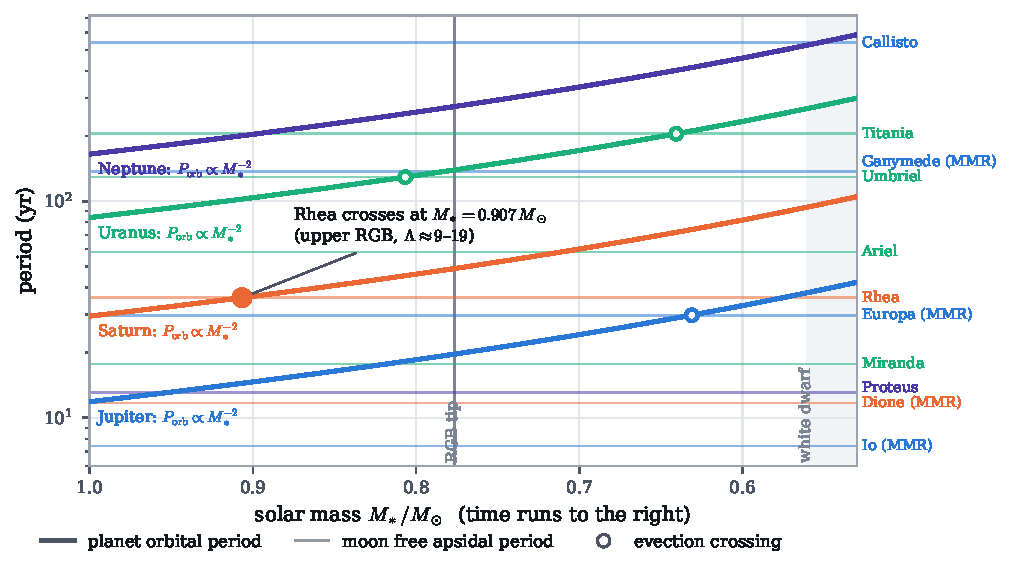
\includegraphics[width=\textwidth]{fig1_sweep.pdf}
\caption{The dying Sun sweeps the evection resonance through the Solar System's moons. Thick curves: planetary orbital periods, which grow as $M_\ast^{-2}$ (Eq.~\ref{eq:adiabatic}). Thin lines: free apsidal periods of the regular moons from Laplace--Lagrange theory. Circles mark crossings before the white-dwarf stage (shaded); the filled circle is Rhea. The vertical line is the RGB tip for $\eta=0.477$.}
\label{fig:sweep}
\end{figure}

\begin{figure}[p]
\centering
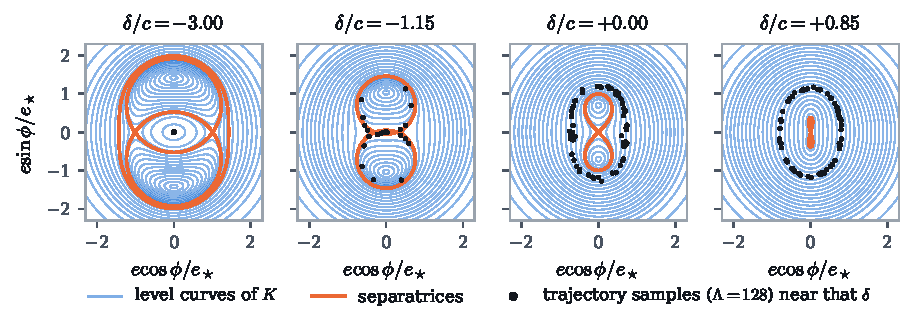
\includegraphics[width=\textwidth]{fig2_portraits.pdf}
\caption{Phase portraits of the normal form at four detunings during a mass-loss sweep ($\eps=3\times10^{-3}$, quadrupole only). Orange: separatrices. Black points: samples of one trajectory ($\Lambda=128$, $e_0=0.01\estar$) near each detuning. As $\delta$ increases the inner region, the resonant lobes and the islands all shrink. The moon is expelled to the outer circulation region and cannot be captured.}
\label{fig:portraits}
\end{figure}

\begin{figure}[p]
\centering
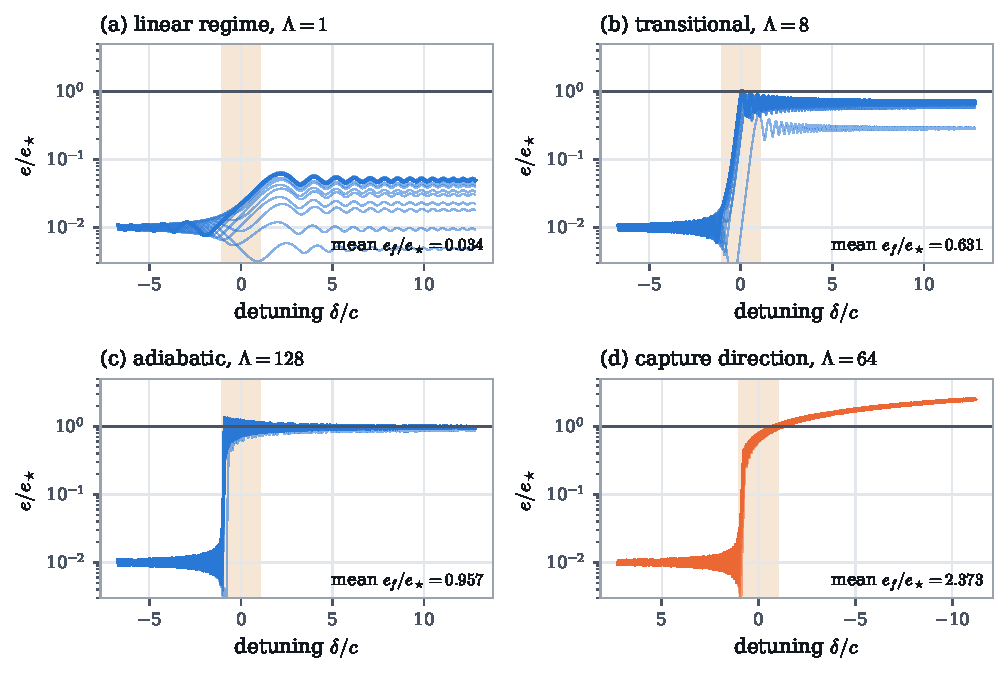
\includegraphics[width=0.95\textwidth]{fig3_timeseries.pdf}
\caption{Eccentricity through the crossing for ensembles of 24 initial phases ($\eps=3\times10^{-3}$, $e_0=0.01\estar$). (a)--(c) Stellar mass loss with increasing adiabaticity; (d) the reverse sweep (inward migration) for comparison, where every member is captured and pumped. Shaded: the parametric band $|\delta|<c$.}
\label{fig:timeseries}
\end{figure}

\begin{figure}[p]
\centering
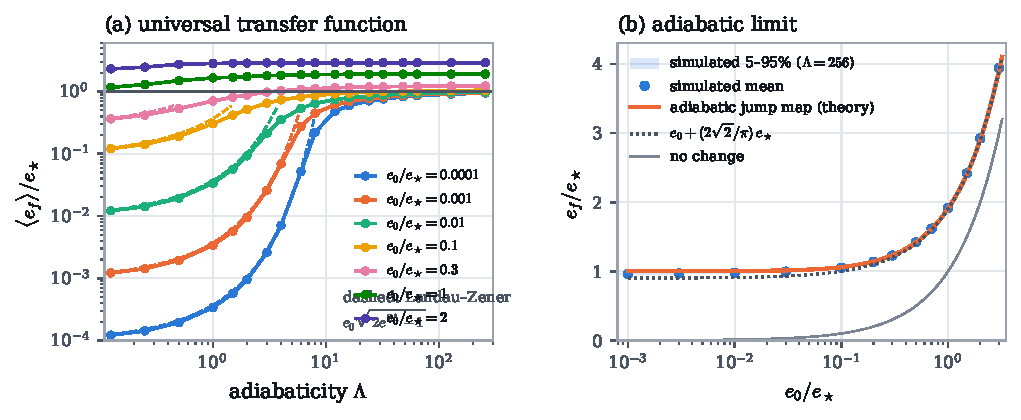
\includegraphics[width=\textwidth]{fig4_transfer.pdf}
\caption{(a) Universal transfer function: mean final eccentricity against $\Lambda$ for initial eccentricities $10^{-4}$--$2\estar$ (points), with the Landau--Zener prediction Eq.~\eqref{eq:LZ} (dashed). (b) Adiabatic limit ($\Lambda=256$): simulated means and 5--95\% ranges against the jump map Eq.~\eqref{eq:jumpmap} and its asymptote Eq.~\eqref{eq:limits}.}
\label{fig:transfer}
\end{figure}

\begin{figure}[p]
\centering
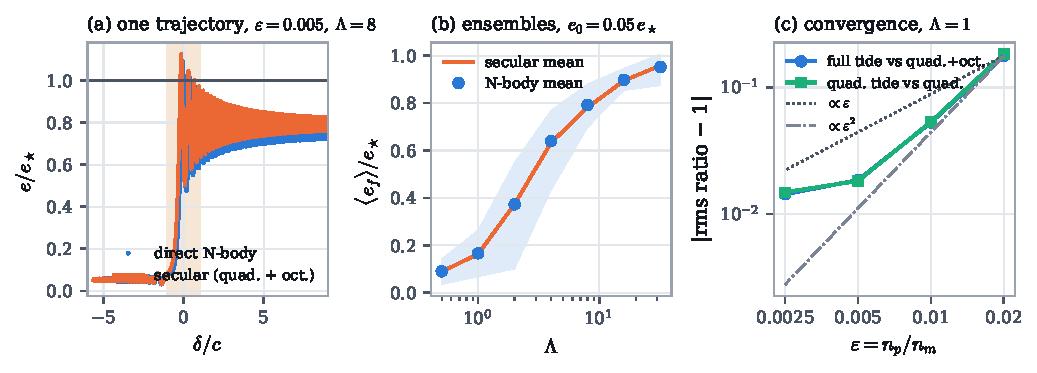
\includegraphics[width=\textwidth]{fig5_nbody.pdf}
\caption{Validation against direct three-body integrations with mass loss. (a) One trajectory ($\eps=0.005$, $\Lambda=8$, $e_0=0.05\estar$). (b) Ensemble means (points; band: 10--90\%) against the secular model (line). (c) Relative rms difference in the linear regime ($\Lambda=1$, 12 phases) against $\eps$, for the full tide (vs.\ quadrupole + octupole) and the quadrupole tide (vs.\ quadrupole), with $\propto\eps$ and $\propto\eps^2$ guides. The last point is at the level of the 12-phase sampling noise.}
\label{fig:nbody}
\end{figure}

\begin{figure}[p]
\centering
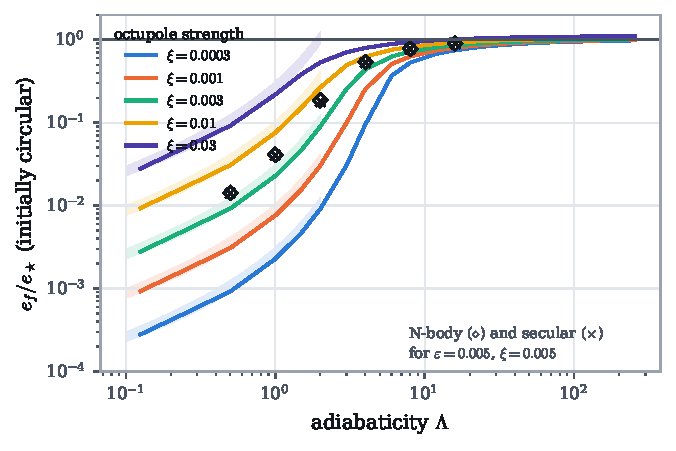
\includegraphics[width=0.7\textwidth]{fig6_octupole.pdf}
\caption{Initially circular moons are seeded by the octupole (parallactic) tide. Lines: secular model for octupole strengths $\xi$; shaded: the seed of Eq.~\eqref{eq:seed} times the rms and maximum Landau--Zener gains. Diamonds: direct $N$-body; crosses: secular model at the same parameters.}
\label{fig:octupole}
\end{figure}

\begin{figure}[p]
\centering
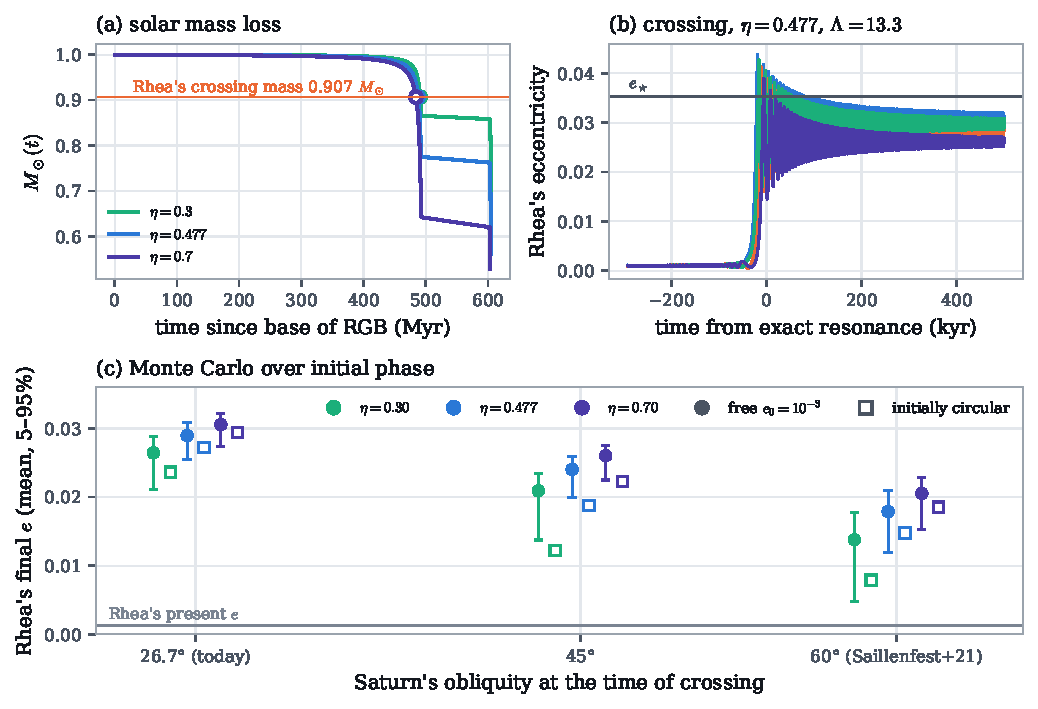
\includegraphics[width=\textwidth]{fig7_rhea.pdf}
\caption{Rhea. (a) Semi-analytic solar mass-loss histories for three Reimers efficiencies; circles mark the crossing. (b) Rhea's eccentricity through the crossing for four initial phases. (c) Final eccentricity against Saturn's obliquity at the time (filled: free $e_0=10^{-3}$; open: circular start).}
\label{fig:rhea}
\end{figure}

\begin{figure}[p]
\centering
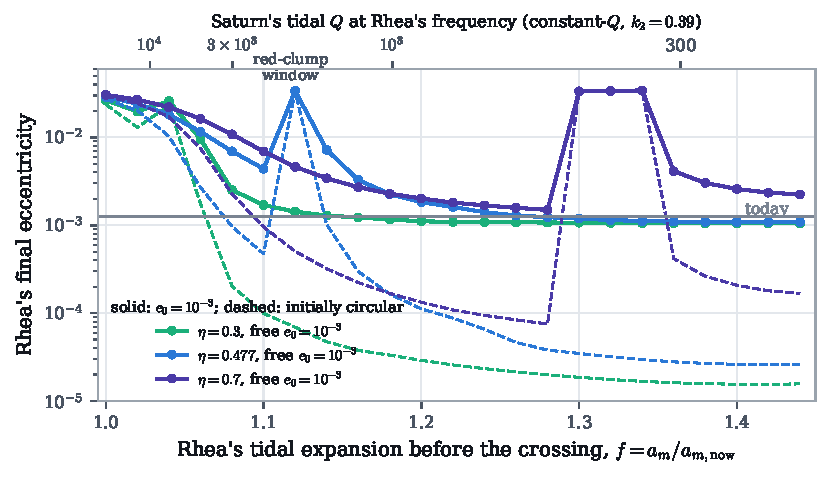
\includegraphics[width=0.85\textwidth]{fig9_race.pdf}
\caption{Tides versus wind. Rhea's final eccentricity against its tidal expansion before the crossing. Top axis: the equivalent constant tidal $Q$ of Saturn at Rhea's frequency (Eq.~\ref{eq:migration}). Small expansions place the crossing on the slow RGB wind (full imprint); larger ones place it on the AGB superwind (weak kick), except in narrow red-clump windows.}
\label{fig:race}
\end{figure}

\begin{figure}[p]
\centering
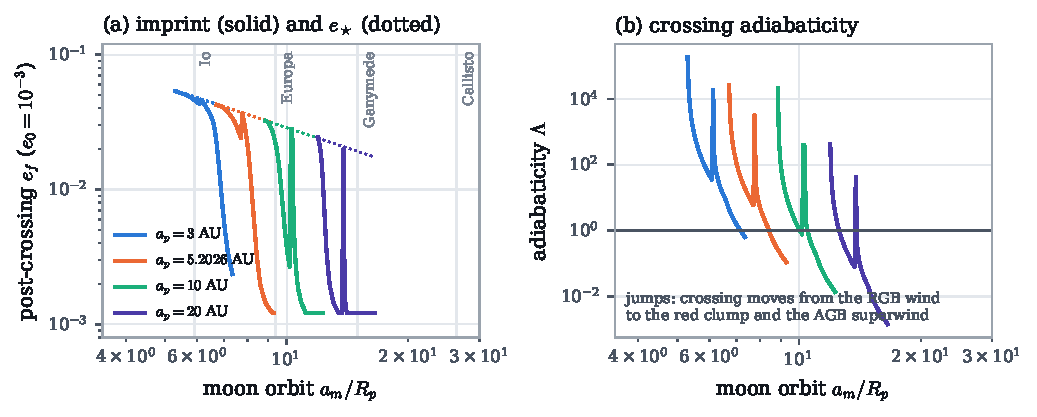
\includegraphics[width=\textwidth]{fig8_exomoons.pdf}
\caption{Exomoons of a Jupiter analogue ($J_2=0.0147$) around a $1\,\msun$ star ($\eta=0.477$). (a) Post-crossing eccentricity (solid) and the universal imprint $\estar$ (dotted) along the swept band for four main-sequence orbital distances; the present Galilean orbits are marked. (b) Adiabaticity of the crossing; the jumps occur where the crossing moves from the RGB wind to the red clump and the AGB superwind.}
\label{fig:exo}
\end{figure}

\clearpage
\appendix

\section{Obliquity factors}\label{app:obliquity}

Let the satellite orbit lie in the planet's equator, inclined by $\theta$ to the planet's orbit, and measure longitudes from the line of nodes. The unit vector to the star has in-plane components $(s_x,s_y)=(\cos\lambda,\cos\theta\sin\lambda)$, so that
\begin{equation}
s_x+is_y=C_+e^{i\lambda}+C_-e^{-i\lambda},\qquad C_\pm=\tfrac12(1\pm\cos\theta).
\end{equation}
The in-plane anisotropic part of the quadrupole is proportional to $(s_x^2-s_y^2)\cos2\varpi'+2s_xs_y\sin2\varpi'$, i.e.\ to the real part of $(s_x+is_y)^2e^{-2i\varpi}$, with
\begin{equation}
(s_x+is_y)^2=C_+^2e^{2i\lambda}+2C_+C_-+C_-^2e^{-2i\lambda}.
\end{equation}
The resonant harmonic $e^2\cos2(\varpi-\lambda)$ therefore carries $C_+^2=\cos^4(\theta/2)$. The term $C_-^2$ has argument $2(\varpi+\lambda)$ and the term $2C_+C_-$ has argument $2\varpi$; both are non-resonant. The axisymmetric part carries $\langle s_x^2+s_y^2\rangle_\lambda=1-\tfrac12\sin^2\theta$, which gives $f_\theta=(3\cos^2\theta-1)/2$.

For the octupole, write $u=\hat{\bm s}\cdot\hat{\bm r}=s_\perp\cos(\theta_r-\chi)$, where $s_\perp e^{i\chi}=s_x+is_y$ and $\theta_r$ is the satellite's longitude. Since $\cos^3x=\tfrac34\cos x+\tfrac14\cos3x$, the first-harmonic part of $P_3(u)=\tfrac12(5u^3-3u)$ is $\big(\tfrac{15}{8}s_\perp^3-\tfrac32s_\perp\big)\cos(\theta_r-\chi)$. Averaging over the orbit with $\langle(r/a)^3\cos f\rangle=-\tfrac52e$ leaves terms in $e\cos(\varpi-\chi)$. Projecting $s_\perp^3e^{i\chi}=(s_x^2+s_y^2)(s_x+is_y)$ and $s_\perp e^{i\chi}$ on $e^{i\lambda}$ gives $C_+^3+2C_+C_-^2$ and $C_+$ respectively. Normalizing by the value $\tfrac{15}{8}-\tfrac32=\tfrac38$ at $\theta=0$ gives Eq.~\eqref{eq:foct}.

\section{Separatrix areas}\label{app:areas}

For $\delta=-qc$ with $q>1$ the separatrix through the hyperbolic points $x_1$ satisfies $\beta x^2+(\delta+c\cos2\phi)x+(\delta+c)^2/4\beta=0$, whose roots are $x_{\rm in,out}=[-(\delta+c\cos2\phi)\mp\sqrt{D}]/2\beta$ with $D=4c\sin^2\phi\,(|\delta|-c\cos^2\phi)$. Hence $A_{\rm in}+A_{\rm out}=\oint-(\delta+c\cos2\phi)\,\dd\phi/\beta=2\pi|\delta|/\beta$ and
\begin{equation}
A_{\rm out}-A_{\rm in}=\frac{8\sqrt c}{\beta}\int_0^1\sqrt{|\delta|-cu^2}\,\dd u=\frac{4}{\beta}\Big[\sqrt{c(|\delta|-c)}+|\delta|\arcsin\sqrt{c/|\delta|}\Big],
\end{equation}
which gives Eq.~\eqref{eq:areas}. At $q=1$, $A_{\rm in}=0$ and $A_{\rm out}=2\pi c/\beta$, so $e_f^2=A_{\rm out}/\pi=2c/\beta=\estar^2$.

\end{document}
